\documentclass[journal,12pt,twocolumn]{IEEEtran}
\usepackage{cite}
\usepackage{amsmath,amssymb,amsfonts,amsthm}
\usepackage{algorithmic}
\usepackage{graphicx}
\usepackage{textcomp}
\usepackage{xcolor}
\usepackage{txfonts}
\usepackage{listings}
\usepackage{enumitem}
\usepackage{mathtools}
\usepackage{float}
\usepackage{gensymb}
\usepackage{comment}
\usepackage[breaklinks=true]{hyperref}
\usepackage{tkz-euclide} 
\usepackage{listings}
\usepackage{gvv}                                        
\def\inputGnumericTable{}                                 
\usepackage[latin1]{inputenc}                                
\usepackage{color}                                            
\usepackage{array}                                            
\usepackage{longtable}                                       
\usepackage{calc}            
\usepackage{multirow}                                         
\usepackage{hhline}                                           
\usepackage{ifthen}                                           
\usepackage{lscape}

\newtheorem{theorem}{Theorem}[section]
\newtheorem{problem}{Problem}
\newtheorem{proposition}{Proposition}[section]
\newtheorem{lemma}{Lemma}[section]
\newtheorem{corollary}[theorem]{Corollary}
\newtheorem{example}{Example}[section]
\newtheorem{definition}[problem]{Definition}
\newcommand{\BEQA}{\begin{eqnarray}}
\newcommand{\EEQA}{\end{eqnarray}}
\newcommand{\define}{\stackrel{\triangle}{=}}
\theoremstyle{remark}
\newtheorem{rem}{Remark}

\begin{document}

\bibliographystyle{IEEEtran}
\vspace{3cm}

\title{NCERT Discrete - 11.9.3.11}
\author{EE23BTECH11037 - M Esha$^{*}$}

\maketitle
\newpage
\bigskip

\renewcommand{\thefigure}{\theenumi}
\renewcommand{\thetable}{\theenumi}

\vspace{3cm}
\textbf{Question 11.9.3.11:} 
Evaluate $\sum_{k=1}^{11} (2 + 3^k)$.

\solution
\begin{table}[h!]
  \centering
  \begin{tabular}{|c|c|c|}
   \hline
   variable&value&description  \\
   \hline
   $x(0)$ & $3$ & first term of the geometric progession\\
   \hline
   $r$ & $3$ & common ratio of the geometeric progression\\
   \hline
   $x(n)$ & $3^{n}u\brak{n}$& $n^{th}$ term of the geometric progession\\
   \hline
   $y(n)$ &$\frac{x(0)(r^{n+1}-1)}{r-1}u\brak{n}$ &Sum of the n term of the geometric progression\\
   \hline 
\end{tabular}


  \caption{Input Parameters}
    \label{tab:table1}
\end{table}

\begin{align}
\sum_{k=1}^{11} (2 + 3^k) 
&= 2(n+1) + \sum_{n=0}^{10}3^{n+1} &= x_o(n)\\
\end{align}

Applying Z-transform:
\begin{align}
X\brak{z} &= x\brak{0}\brak{\frac{1}{1-rz^{-1}}}, \quad{|rz^{-1}|<1} \\
y\brak{n} &= x\brak{n}*u\brak{n} \\
Y\brak{z} &= X\brak{z}U\brak{z}\\
&=3\brak{\frac{1}{1-3z^{-1}}}\brak{\frac{1}{1-z^{-1}}} ,\quad{|z|>3}\\
&=\brak{\frac{3}{2}}\brak{\brak{\frac{3}{1-3z^{-1}}}-\brak{\frac{1}{1-z^{-1}}}}\\
\frac{1}{1-rz^{-1}} &\xleftrightarrow{\mathcal{Z}^{-1}}  r^nu(n), \quad{|z|>r}\\
y\brak{n} &= 3\brak{\frac{3^{n+1}-1}{3-1}}u(n) \\
y\brak{n} &= \brak{\frac{3^{12}-1}{2}}\\
y_o(n)= 2(n+1)+y\brak{n}
\end{align}
\begin{figure}[h!]
    \centering
    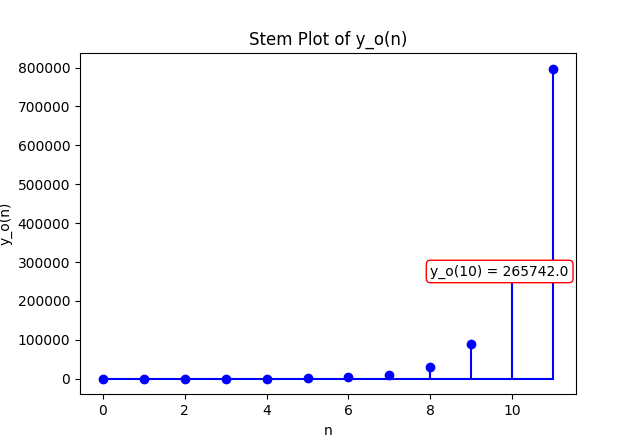
\includegraphics[width=\columnwidth]{11/9/3/11/figs/11.png}
    \caption{stem plot }
    \label{fig:1}
\end{figure}

\end{document}

